\documentclass[10pt,a4paper]{article}
\usepackage{amsmath}
\usepackage{amssymb}
\usepackage{amsthm}
\usepackage{enumerate}
\usepackage{fancyhdr}
\usepackage{graphicx}
\usepackage{hyperref}
\usepackage[utf8]{inputenc}
\usepackage[a4paper, top=1in, bottom=1.25in, left=0.75in, right=0.75in]{geometry}

\begin{document}
\pagestyle{fancy}
\fancyhead[R]{Robert Schüle 319782, Christoph Ende 331655}

%%%%%%%%%%%%%%%%%%%%%%%%%%%%%%%%%%%%%%%%%%%%%%%%%%%%%%%%%%%%%%%%%%%%%%%%%%%%%%%%
\subsection*{8.1 Binomial Coefficients}

\begin{eqnarray}C_{(p,N)}\;+\;C_{(p,N-1)}\;&=&\;C_{(p+1,N)} \\
2 \sum_{k=0}^{N-1} {p-1 \choose k} \;+\; 2 \sum_{k=1}^{N-1} {p-1 \choose k-1} \;&=&\; 2 \sum_{k=0}^{N-1} {p \choose k} \;\;\;\Big{|}\mbox{\small{extend k range in $2^{nd}$ sum:}} {n \choose -1} = 0\; \forall\; n \in \mathbb{N} \\
2 \sum_{k=0}^{N-1} {p-1 \choose k} \;+\; 2 \sum_{k=0}^{N-1} {p-1 \choose k-1}  \;&=&\; 2 \sum_{k=0}^{N-1} {p \choose k} \\
2 \sum_{k=0}^{N-1}\Big{[} {p-1 \choose k} \;+\; {p-1 \choose k-1} \Big{]} \;&=&\; 2 \sum_{k=0}^{N-1} {p \choose k} \;\;\;\Big{|} \; \mbox{\small{apply (2) from task sheet}} \\
2 \sum_{k=0}^{N-1} {p \choose k} \;&=&\; 2 \sum_{k=0}^{N-1} {p \choose k}_{\tiny{\qed}}
\end{eqnarray}
\noindent

%%%%%%%%%%%%%%%%%%%%%%%%%%%%%%%%%%%%%%%%%%%%%%%%%%%%%%%%%%%%%%%%%%%%%%%%%%%%%%%%
\subsection*{8.2 Geometry of Linear Classification}
\begin{enumerate}[a)]
\item
The decision boundary is a hyperplane defined by $(w^Tx - b = 0)$. $w$ decides the orientation,
$b$ the offset from the origin. $w$ points in the direction of positive classification values $y(x)$ (\ref{820}).
\begin{figure}[h]
	\centering
	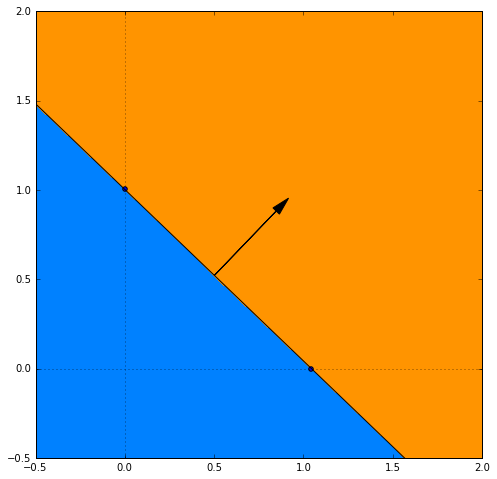
\includegraphics[width=0.6\textwidth]{820.png}
    \caption{}
	\label{820}
\end{figure}
\begin{itemize}
\item the decision boundary is given by $\{x\;|\;y=0\}$
\item this can be expressed as a linear function: $x_1 = \;-\frac{w_0}{w_1}x_0 \;-\; \frac{b}{w_1}$
\item as one can see, the slope of the boundary is $\;-\frac{w_0}{w_1}$ and the offset is $\;-\frac{b}{w_1}$
    \item figure \ref{821}: $w_0$ only affects the slope
    \item figure \ref{822}: varying $w_1$ also results in different offsets
    \item figure \ref{823}: increasing $b$ leads to a negative offset, scaled by $w_1$
\end{itemize}
\begin{figure}[h]
	\centering
	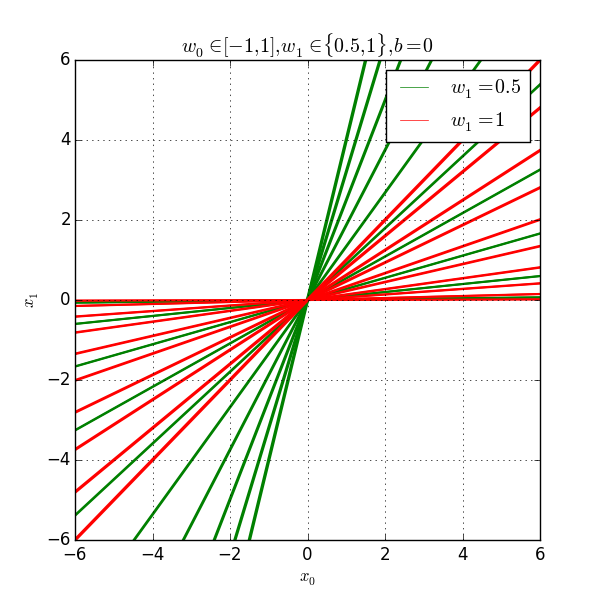
\includegraphics[width=0.6\textwidth]{821.png}
    \caption{}
	\label{821}
\end{figure}
\begin{figure}[h]
	\centering
	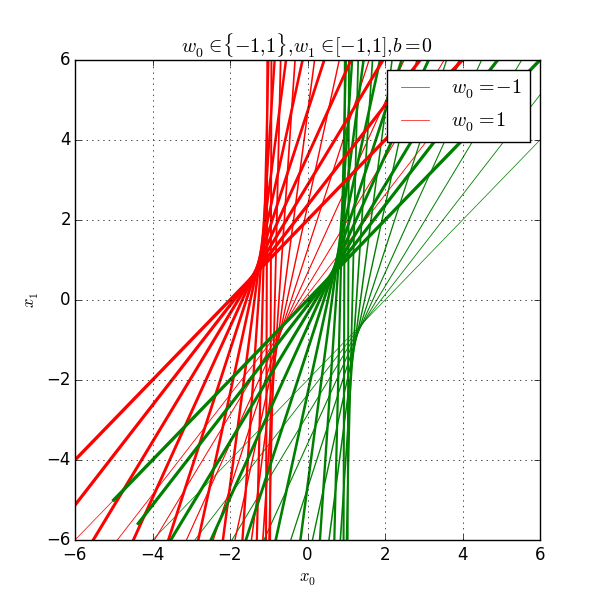
\includegraphics[width=0.6\textwidth]{822.png}
    \caption{}
	\label{822}
\end{figure}
\begin{figure}[h]
	\centering
	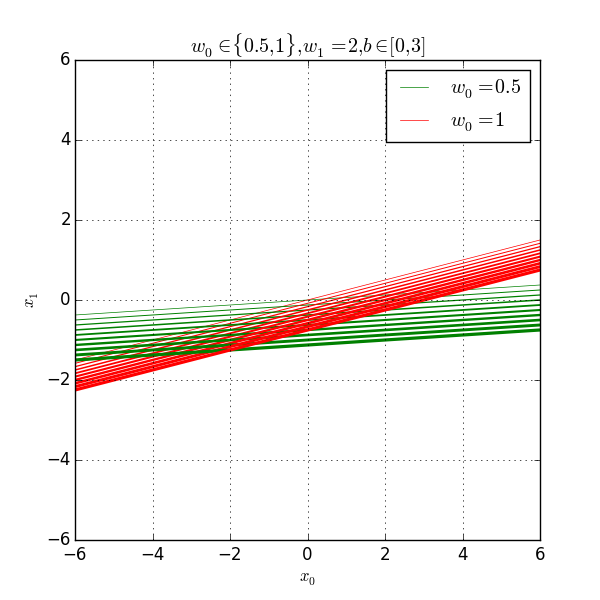
\includegraphics[width=0.6\textwidth]{823.png}
    \caption{}
	\label{823}
\end{figure}

\item
A linear classifier divides the input space into two half-spaces. The \textit{shattering coefficient} $s_{halfspaces}(n)$ then is the largest number of subsets that can be formed by intersecting \textit{any} one input set $X$ of $n$ points using half-spaces. The highest possible shattering coefficient is $2^{n}$.

$s_{H}(n) = \underset{X \subseteq \Omega \\ |X| = n}{max}\ |\{X \cap H_i \mid H_i \in H\}|$

The \textit{VC-dimension} $d_{VC}$ provides an upper bound to the shattering coefficient: $ln(s(n)) \leq d_{VC}(1+ln\frac{p}{d_{VC}})$.
It provides a measure of the capacity of the separation capabilities of the separator function class H. If we can find n points, that can be shattered by H (that is, H can separate all possible binary labelings of the points), then VC(H) = n. It is sufficient, that some such example of n points exists (fixed points, but H must shatter them for all possible labelings).

Small VC-dimensions are often applicable for real life data, since close points will have same labels, so separator classes with low VC-dimensions (low complexity models) might actually be preferrable. For a linear classifier in 2 input dimensions, the VC-dimension is 2.
Correct linear classification is possible, if all classes can be bounded by non-overlapping convex domains.

\end{enumerate}
\clearpage
%%%%%%%%%%%%%%%%%%%%%%%%%%%%%%%%%%%%%%%%%%%%%%%%%%%%%%%%%%%%%%%%%%%%%%%%%%%%%%%%
\subsection*{8.3 The primal SRM problem}
\begin{enumerate}[a)]
\item
The margin is the lowest distance between the decision boundary and the closest datapoints. The margin of a canonical hyperplane is set to be $d = \frac{1}{|w|}$ by choosing $|w|$ appropriately.
A low margin means higher model complexity $C$, which means we might get a worse upper bound for the generalization error $E^G < E^T + C$, even if the separate the training set perfectly (overfitting).
A high margin reduces model complexity, but increases the training error (underfitting).
\item
Idea: Project $x$ on $w$, which gets us the large vector from the origin to the tip of the dotted line in figure~\ref{fig:sketch}}. From this we have to subtract the length of the part from the origin to the decision boundary, which will be  $\alpha$.
\begin{figure}[h]
	\centering
	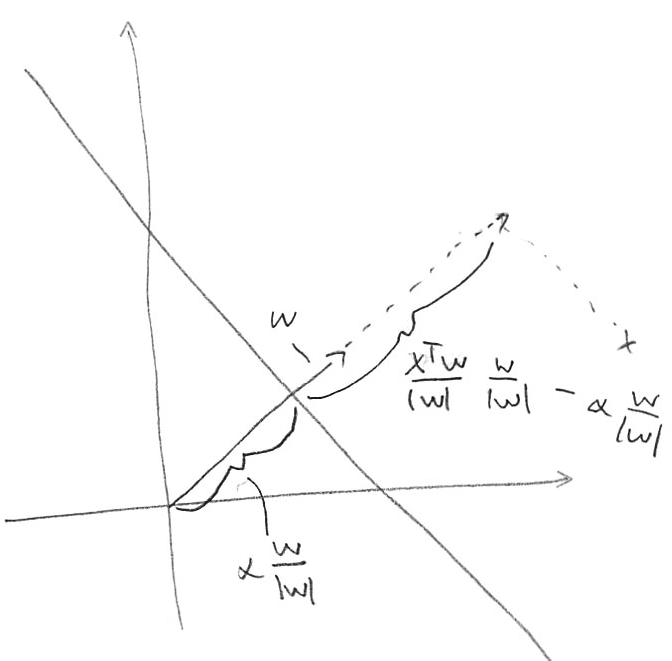
\includegraphics[width=0.5\textwidth]{sketch}
	\caption{sketch for 8.3b}
	\label{fig:sketch}
\end{figure}

Let $x$ be any closest point.
The projection of $x$ onto $w$ is is $\frac{x^Tw}{|w|} \frac{w}{|w|}$, where $\frac{w}{|w|}$ is a unit vector.

Calculate $\alpha$ (the scalar to stretch $\frac{w}{|w|}$ by to reach the boundary):
\begin{align*}
	& w^T(\alpha \frac{w}{|w|}) + b = 0 \\
	\Leftrightarrow\ & \frac{\alpha}{|w|}w^T(w) + b = 0 \\
	\Leftrightarrow\ & \frac{\alpha}{|w|}\underbrace{w^Tw}_{|w|^2} + b = 0 \\
	\Leftrightarrow\ & \frac{\alpha}{|w|}|w|^2 + b = 0 \\
	\Leftrightarrow\ & \alpha|w| + b = 0 \\
	\Leftrightarrow\ & \alpha = \frac{-b}{|w|}
\end{align*}

Then the distance of $x$ to the decision boundary is:
\begin{align*}
	d=\ & \left\Vert\frac{x^Tw}{|w|} \frac{w}{|w|}\right\Vert - \left\Vert\alpha \frac{w}{|w|}\right\Vert \\
	=\ & \frac{x^Tw}{|w|} - \frac{-b}{|w|} \\
	=\ & \frac{x^Tw + b}{|w|} \qquad\left\vert \text{for the closest point: } w^Tx + b = 1\\
	=\ & \frac{1}{|w|} \\
\end{align*}

For points farther away than $x$ the term $\frac{x^Tw}{|w|} \frac{w}{|w|}$ increases, while $\alpha \frac{w}{|w|}$ stays the same. Hence the distance gets larger, so overall: $d \geq \frac{1}{|w|}$

\item
Primal Problem:

minimize $f_{0}(x)$ subject to $f_{k}(x) \leq 0$, $k=1,...,m$, which in our case is:

minimize $\frac{1}{2}|w|^2$ subject to $-y_T^{(\alpha)}((w^Tx^{(\alpha)}+b)-1) \leq 0$

This means we wish to find the largest margin $\frac{1}{|w|}$, that seperates all training datapoints:

$y_T^{(\alpha)}(w^Tx^{(\alpha)} + b) \geq 1 \quad \forall \alpha$

holds for
$y_T^{(\alpha)} \in \{-1, 1\}, \quad \forall \alpha$ and

$ w^Tx^{(\alpha)} + b \geq y_T^{(\alpha)} \quad \forall y_T^{(\alpha)} = 1$,

$ w^Tx^{(\alpha)} + b \leq y_T^{(\alpha)} \quad \forall y_T^{(\alpha)} = -1$

The constraint term at the top is just a concise rewrite of these 2 inequalities.

Since the objective function $\frac{1}{2}|w|^2$ is convex, it only has one optimal solution. And since this is a standard formulation, we can use solvers to solve it.
The solution should classify all training points perfectly ($E^T = 0$), while minimizing the complexity $C$.

\end{enumerate}
%%%%%%%%%%%%%%%%%%%%%%%%%%%%%%%%%%%%%%%%%%%%%%%%%%%%%%%%%%%%%%%%%%%%%%%%%%%%%%%%
\subsection*{8.5 Kernel Construction}
\begin{enumerate}[a)]
\item kernel matrix is symmetric:
\begin{eqnarray}
K(x,x')\;=\;\phi(x)^T\,\phi(x')\;=\;\phi(x')^T\,\phi(x)\;=\;K(x',x)
\end{eqnarray}
\item kernel matrix is positive semidefinite:
\begin{eqnarray}
a^T K a\;=\;\sum^P_{i,j=0} a_i a_j K_{ij}\;=\;\sum^P_{i,j=0}a_i a_j \langle \phi(x_i), \phi(x_j) \rangle \\
= \langle\; \sum^P_{i=0}a_i \phi(x_i) \;,\; \sum^P_{j=0} a_j \phi(x_j)\;\rangle \;=\; || \sum_{i=0}^P a_i \phi(x_i) ||^2 \;\geq\;0
\end{eqnarray}
\item sum of two kernels is also a valid kernel:
\begin{itemize}
\item the sum of two symmetric matrices is (obviously) also symmetric and the sum of two positive semidefinite matrices is positive semidefinte as well:
\end{itemize}
\begin{eqnarray}
a^T (K_1\;+\;K_2) a\;=\;a^T K_1 \,a\;+\;a^T K_2 \,a\;=\;c_1\;+\;c_2\;\geq\;0
\end{eqnarray}
\begin{itemize}
\item this makes the sum of those matrices also a valid kernel, as Mercer's theorem states (Haykin - \textit{"Neural Networks - A Comprehensive Foundation"},$\;2^{\mbox{\tiny{nd}}}$ Ed., p. 331)
\end{itemize}
\end{enumerate}

\end{document}
